\newif\ifcommentenabled \commentenabledtrue
\newcommand{\TS}[1]{\ifcommentenabled\textcolor{red}{TS: #1}\fi}
\newcommand{\TK}[1]{\ifcommentenabled\textcolor{blue}{TK: #1}\fi}

\documentclass[12pt, a4paper, titlepage]{report}
\usepackage[cache=false]{minted} % highlight programming languages
\usepackage[dvipdfmx]{graphicx}
\usepackage[nottoc,numbib]{tocbibind}
\usepackage[utf8]{inputenc}
\usepackage{amsmath}
\usepackage{color}
\usepackage{enumerate}
\usepackage{hyperref}
\usepackage{bussproofs}
\usepackage{mathptmx}
\usepackage{mathpartir} % automatically fit multiple math expressions
\usepackage{pdfpages} % PDF inclusion
\usepackage{verbatim} % comment environment
\hypersetup{
  colorlinks = true,
  linkcolor = cyan
}

% Title Page
\title{Bachelor Thesis \\ TODO: TITLE}
\author{
  03190413 Takemaru Kadoi
  \\[1cm]
  {\small Supervisor: Prof. Masahiro Fujita},
  {\small Advisor: Assistant Prof. Taro Sekiyama}
  \\[1cm]
  {\small University of Tokyo, Department of Information and Communication Engineering}
}
\date{\today}

\begin{document}

% front page
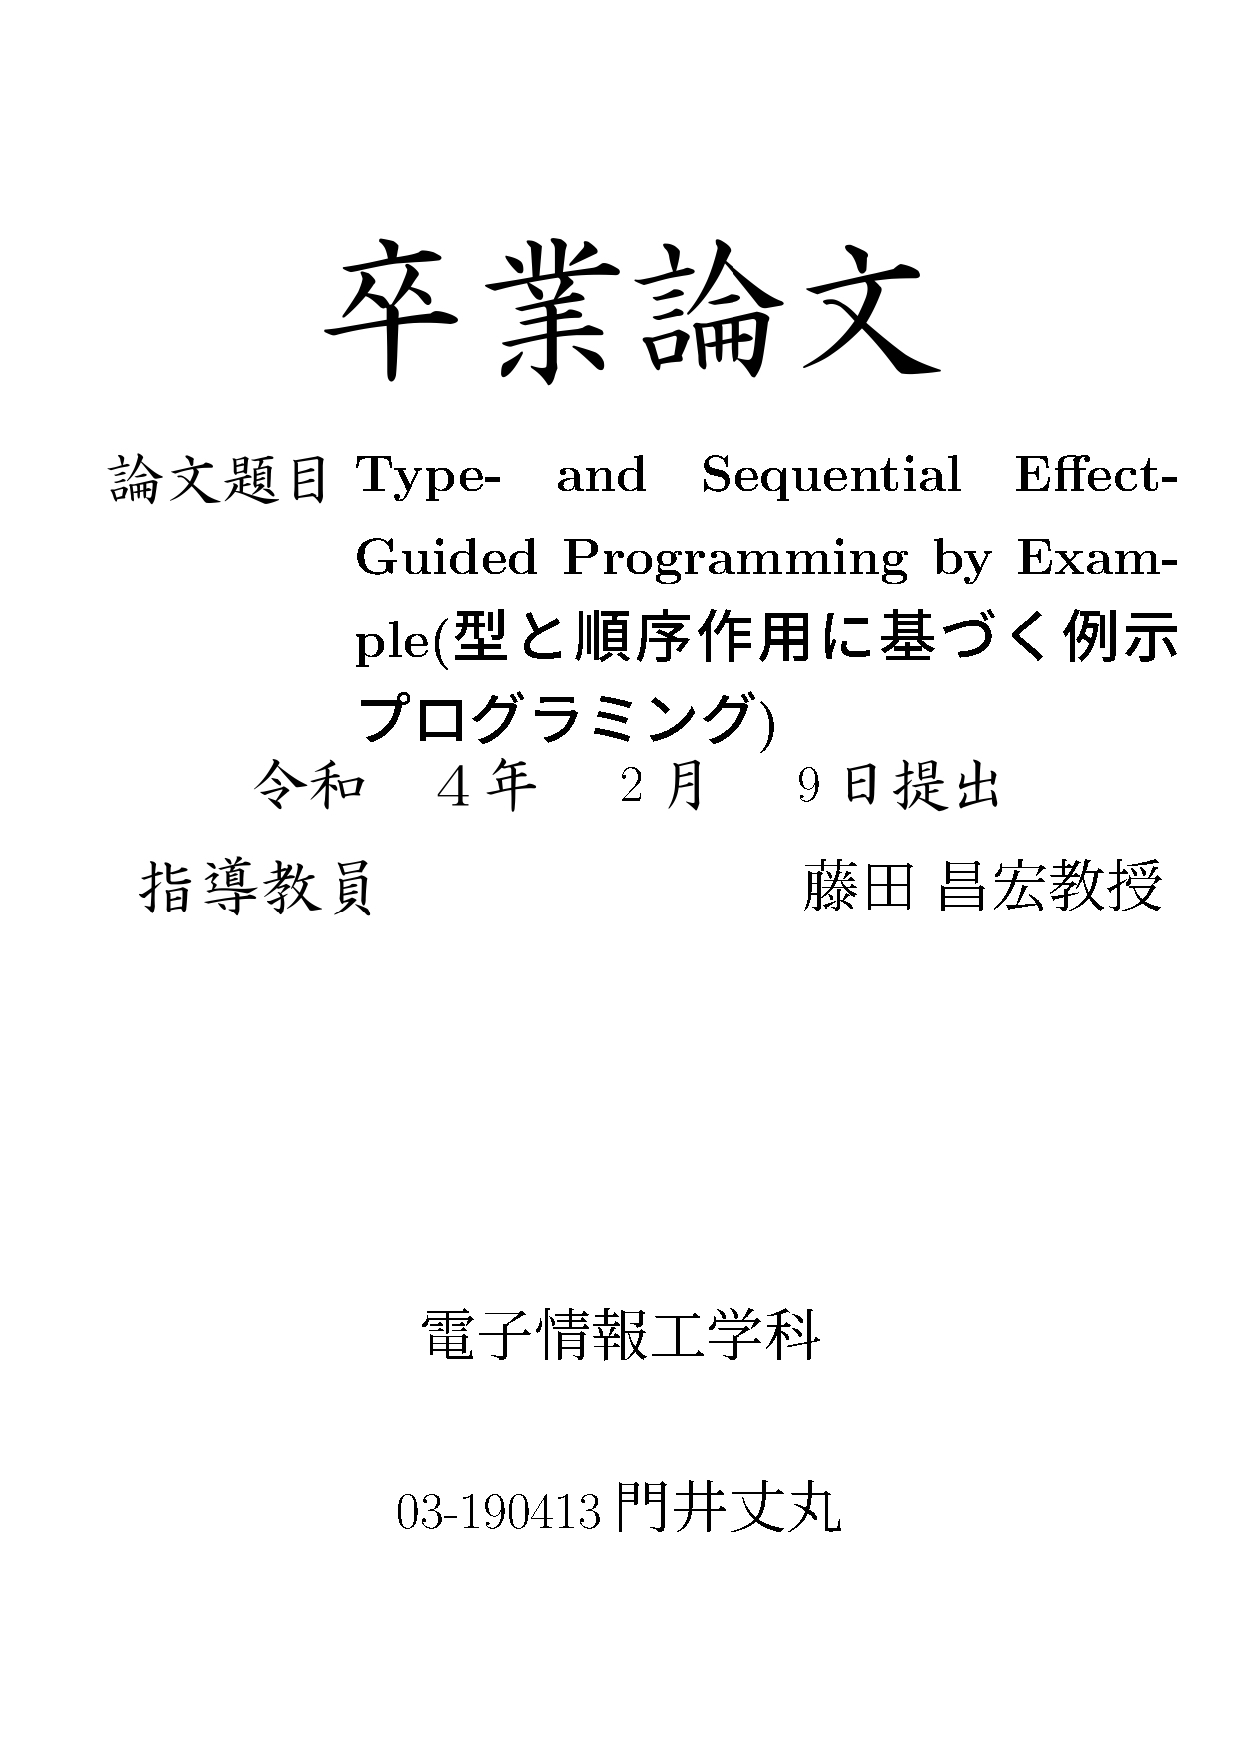
\includepdf[pages={-}]{images/sotsuronFront.pdf}

% header
\maketitle
\newpage
\tableofcontents
\newpage

\chapter*{Acknowledgment}
This research was supervised by Prof. Fujita at the University of Tokyo and supported by Assistant Prof. Sekiyama at National Institute of Technology. \\
I thank my colleagues at the University of Tokyo, Miyasaka-san, Koike-san, Yu-san, Nagasawa-san, and Yi-san.
% TODO: add twitter accounts
I also show my gratitude to my good friends, hnkz, Akio, Saeki, Arahata, Hori, Naito, Chen, and Sakura.

% overview of the research topic
\chapter{Abstract} \label{chapter:abstract}
In recent years, several tools have been developed to enhance the productivity of programmers.
In particular, tools for generating code have attracted a lot of attention, and program synthesis is a research field that supports this development.
Program synthesis requires specifications with which users tell a computer what they want to achieve.
In the case of logical formulae \TS{expressions $\rightarrow$ formulas / formulae} \TK{use "formulae" instead of "expressions".}, it is
difficult for programmers who are not skilled in math while its strictness contributes to accurate code generation. \TS{The advantages of logical formulas should be described.} \TK{add an explanation about its strictness.}
With natural language, computers may not be able to understand the meaning, and the intention may not be conveyed correctly even though programmers can find it easy to write specifications. \TS{What are the advantages of specifications in natural languages?} \TK{add an explanation about its human friendly character.}
This paper examines the use of a type and effect system as a specification that is easy to understand by both humans and computers alike. The types are properties of data and can be used to describe the input and output of a function. The effects, which can explain the internal processes of a function, represent a transition in a state, such as the value of a variable, shared memory between threads, and I/O operations.
\TS{What are types and effects?} \TK{add explanations}
Types are familiar to programmers who use statically typed languages.
Many users are unfamiliar with effects, but the effects \TS{What "they" means is a bit ambiguous. It is clearer to say "effects".} \TK{use "effects".}can describe the internal behavior of programs \TS{Here is the first place you mention functions, so it sounds abrupt.  It may be natural to say "code" or "programs"} \TK{use "code".}and are easy to understand if designed properly.
By utilizing type and effect, I can efficiently explore candidate code and demonstrate that the intended code will be generated. I will demonstrate some specifications and an example of a program that has been generated based on these specifications.
\TS{(DONE)How do you synthesize programs with types and effects?  What experiments are (planed to be) conducted?  How about results?} \TK{describe how to synthesize and what to do.}

In Chapter \ref{chapter:introduction}, I discuss the motivation for this research, what program synthesis is, and existing methods  The details of the existing methods can be discussed in the related work chapter, which should be  put before the conclusion.
I give examples of existing researches in Chapter \ref{chapter:relatedWork}.
I explain my proposed method in Chapter \ref{chapter:method}.
I present in Chapter \ref{chapter:experiment} the results obtained by the proposed method and evaluate them.
Chapter \ref{chapter:conclusion} concludes with a summary of the results and evaluation, as well as future issues.

\chapter{Introduction}\label{chapter:introduction}
\TS{Introduction should include a summary of what this thesis achieves.  The details of the existing methods can be discussed in the related work section, which should be  put before the conclusion.} \TK{move "Related Work"(previous "Existing methods") to after this chapter and add section "Achievement" in this chapter}
  \section{Motivation}
    The purpose of this research is to contribute to programming efficiently and safely in the current software-centric world that demands for many lines of secure code.
    I tackle this problem by using a type-effect system and a technique of program synthesis.
    Bodik insists that this issue is tractable from non-programmers' and programmers' perspectives \cite{bodik:2015}.
    I, however, focus only on a programmer point of view.

    % present situation(type is used in everyday development, generating code is required)
    % what to do(type is usable to boost efficient programming)
    Today, more and more people are developing software.
    Thus, it can be said that an increasing number of people are writing programming languages proportionally.
    As a result of the current situation, the demand for secure code is also increasing.
    Recent software development is facilitated by programming languages that are based on type systems, such as Rust, TypeScript and Scala.
    This shows that the type theory is not only an interesting but also a practical research topic, and modern programmers are familiar with the notion.
    Additionally, the increasing demand illustrates the need for more time-efficient and productive programming.
    The program synthesis fits for this requirement because it is a research topic to deal with easy code generation.

    I am motivated by these trends in my research.
    My goal is to help people develop reliable software easily through the type theory and the program synthesis.
    An additional point that I would like to incorporate into my research is the effect system, which is an informative and descriptive system for programming languages.
    This system allows us to describe the internals of a function, which results in high-quality code generation.
    Namely, we can use the system to generate more secure and intended code than code without it.
    Although this concept is unfamiliar to many programmers, the one in this paper is easily understandable and its popularity is not a big obstacle.

  \section{Program Synthesis}
    In this section, I would like to explain what the program synthesis is for those new to this field.
    Gulwani, Polozov, and Singh summarize it as ``the task of automatically finding a program in the underlying programming language that satisfies the user intent expressed in the form of some specifications'' in their survey paper \emph{``Program Synthesis''} \cite{gulwani:2017}.

    I illustrate the process of the program synthesis below.
    \begin{figure}[htbp]
      \centering
      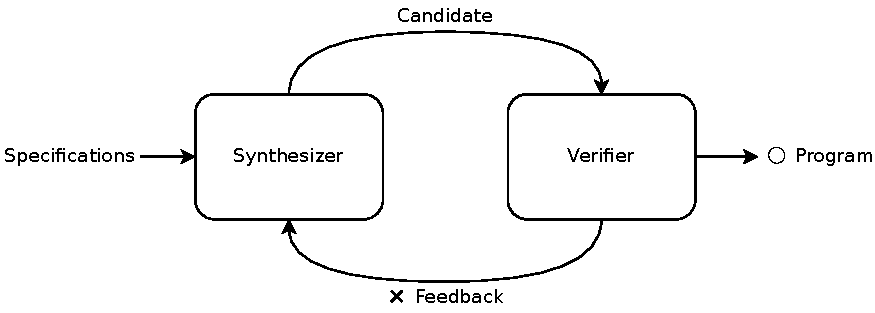
\includegraphics[width=1\textwidth]{images/synthesis.pdf}
      \caption{How the program synthesis generates program}
      \label{synthesisOverview}
    \end{figure}

    The program synthesis consists of 4 steps.
    \begin{enumerate}
      \item To receive specification from a user.
      \item To line up a candidate program.
      \item To check if the candidate program meets some requirements.
      \item To return feedback to the synthesizer or synthesize the program depending on whether it meets the requirements or not
    \end{enumerate}

    Moreover, it has 3 things to consider.
    \begin{enumerate}
      \item User Input
      \item Search Space
      \item Search Technique
    \end{enumerate}
    Synthesizers can accept a variety of inputs.
    Natural languages, logical formulae, and incomplete program code are acceptable forms of communication.
    In relation to the speed and accuracy of program synthesis, search space is a consequential aspect.
    When the target language is a simple language such as brainfuck, which is created by Urban Müller \cite{easter:2020}, the complexity will differ from when the target language is a fully functional language such as C++.
    I have contributed to the field of search technique in this paper.
    The technique is an essential component of the program synthesis process.
    An algorithm determines how fast and how accurately a synthesizer will produce code, and it inseparable from the two factors, user input and search space.

    I am going to deal with these questions in section \ref{section:syntheticProcess}, in which I cover how to synthesize a program.

  \section{Achievement} % contribution of this paper and intro to technical part

\chapter{Related Work}\label{chapter:relatedWork}
  The purpose of this chapter is to provide you with a brief overview of existing search techniques that seem to be relevant. As I said in the previous section, one of the factors that have improved the tractability of search space is new search techniques.
  It is pertinent to note that even though I will describe some techniques as separate ones, they are all interconnected. A type of approach is used by another type of approach and vice versa. This categorization is just to clarify what aspects different algorithms have in common.
  \section{Enumerative Search}
  \section{Constraint Solving}
  \section{Stochastic Search}
  \section{Deduction-based Programming}
  % TODO: add type-driven program synthesis

% my approach to the problem
\chapter{Method}\label{chapter:method}
  \section{Syntax}
    \begin{minted}[breaklines, linenos]{ocaml}
      let _ = print_endline "hello world"
    \end{minted}
    \begin{figure}[htbp]
      \begin{flushleft}
        \textbf{Reduction rules} \quad \framebox{$e_1 \rightarrow e_2$}
      \end{flushleft}
      \begin{center}
        \begin{prooftree}
          \AxiomC{A}
          \UnaryInfC{B}
          \AxiomC{C}
          \BinaryInfC{D}
          \AxiomC{E}
          \AxiomC{F}
          \BinaryInfC{G}
          \UnaryInfC{H}
          \BinaryInfC{J}
          \end{prooftree}
          \hfil
          \begin{prooftree}
            \AxiomC{A}
            \UnaryInfC{B}
            \AxiomC{C}
            \BinaryInfC{D}
            \AxiomC{E}
            \AxiomC{F}
            \BinaryInfC{G}
            \UnaryInfC{H}
            \BinaryInfC{J}
          \end{prooftree}
      \end{center}
    \end{figure}
  \section{Semantics}
    \subsection{Static Semantics} % type-checking rules
    \subsection{Dynamic Semantics} % evaluation rules
  \section{Type and Effect System}
    \cite{pierce:2002}
    \subsection{Type System}
    \subsection{Effect System}
  \section{Synthetic Process}\label{section:syntheticProcess}

% my approach to the problem
\chapter{Experiment}\label{chapter:experiment}
\section{Result}
\section{Consideration}

% qualitative result and remaining problems/future work
\chapter{Conclusion}\label{chapter:conclusion}

\bibliographystyle{unsrt}
\bibliography{
  bib/brainfuck,
  bib/msSynthesis,
  bib/synthesisOp,
  bib/tapl,
}

\end{document}
